\documentclass{standalone}
\begin{document}

\chapter*{Introduction}\addcontentsline{toc}{chapter}{Introduction}
\markboth{Itroduction}{Introduction}


Since the end of 2019, COVID-19 has widely spread all over the world. Up to now the gold standard for the diagnosis of this disease are the reverse transcription-polymerase chain reaction (RT-PCR) and the gene sequencing of sputum, throat swab and lower respiratory tract secretion~\cite{ART:Zhao}.

An initial prospective made by Huang et al. ~\cite{ART:Huang}on chest CT scans of patients affected by COVID-19, has shown the $98\%$ of examined subjects have shown a bilateral patchy shadows or ground glass opacity (GGO) and consolidation(CS). Their severity, shape and involved percentage of lung were made in relation with the stage of the disease~\cite{ART:Bernheim}. In the end, other studies have monitored the change in volume and shape of these features on healed patients~\cite{ART:Ai} in order to check their actual recovery. These behaviour can be seen in \figurename\,\ref{fig:HealthVSCovid}, in which chest CT scans of patient with different severity of disease are compared.

\begin{figure}[h!]
	\centering
	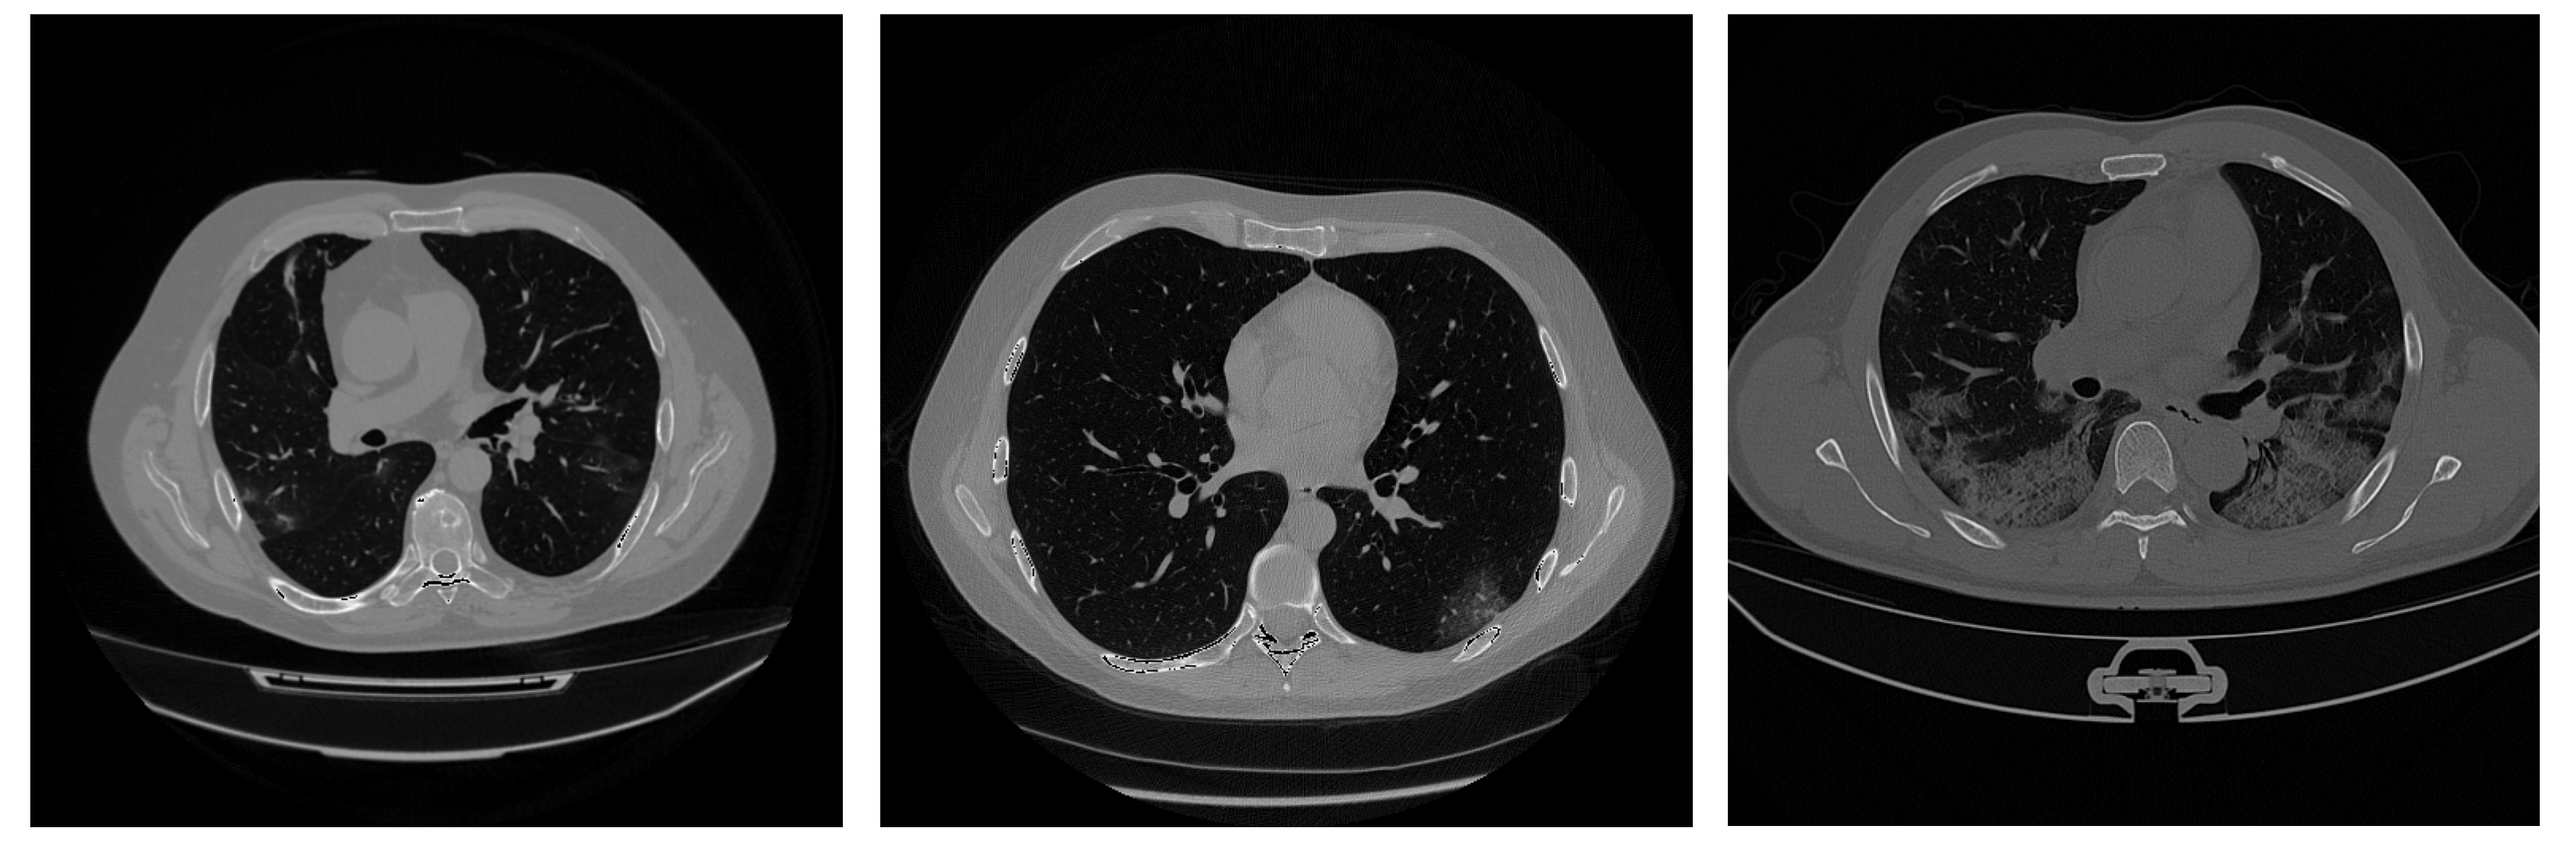
\includegraphics[scale=.37]{lesionStage.png}
	\caption{Groud Glass Opacity and Consolidation on chest CT scans of COVID-19 affected patients with different severity of the disease. From left to right we can observe an increment of the GGO areas in the lung.}\label{fig:HealthVSCovid}
\end{figure} 

GGO and CS are not exclusive of COVID-19, but may be also caused by pulmonary edema, bacterial infection, other viral infection or alveolar haemorrage~\cite{ART:Collins}. The combination between CT scan information and other diagnostic techniques like the RT-PCR mentioned above, may help the diagnosis, the monitoring of the course of the disease and the checking of the recovery in healed patients. The study of these patterns may help to understand the infection pathogenesis, which is not well known since COVID-19 is a new disease.

Identification and quantification of these lesions in chest CT scans is a fundamental task. Up to now the segmentation is made in a manual or semiautomatic way, which are time consuming(several hous or days) and subjected to the operator experience, since involves the interaction with trained personnel. Moreover these kind of segmentation cannot be reproduced. To overcome these issues an automatic and fast way for the segmentation is required.

This work of thesis, made in collaboration with the Department of Diagnostic and Preventive Medicine of the Poloclinico Sant'Orsola - Malpighi, aims to develop an automatic pipeline for the identification of GGO and CS in chest CT of patient affected by COVID-19. The work was based and tested on chest CT scans provided by Sant'Orsola, but also public repositories~\cite{DATA:ZENODO}~\cite{DATA:MOSMED} where used as benchmark.

We start out discussion by understanding what is a digital medical image, its physical meaning and digital representation, focusing mainly on Computed Tomography. After that a brief review on the main image segmentation techniques will be presented,focusing on the ones used for the implementation of the pipeline.

The discussion will continue by describing the main pipeline characteristics and its structure: We will see how color quantization was used to achieve the segmentation and how the digital image properties were used in order to take into account different image features. We also discuss how a preliminary lung segmentation will help the identification performances. After that we will continue the discussion by describing in details the pipeline implementation.

In the end we will discuss the segmentation results. The pipeline performances were checked trough different method, like visual comparison with other segmentation techniques, quantitative comparison against manual annotation and blind evaluation by experts. Also the segmentation achieved on healthy control was considered as benchmark.

\end{document} 